%!TEX root = ../dokumentation.tex

\chapter{Gruppenarbeit}\label{cha:Gruppenarbeit}
Die Aufgabe bestand in der Implementierung einer 2003-Architektur. Da unsere Gruppe aus vier Mitgliedern besteht, wurde eine 2004-Architektur implementiert. Die Implementierte Anwendung
Für die Calculators haben wurde ein Interface entwickelt, welches jeder Calculator implementiert. Dieses Interface bietet eine Methode, um die Ergebnisse der Berechnungen der Calculators abzufragen.
Die Main-Klasse bildet den Einstiegspunkt des Programms und bündelt die Funktionalität zum Aufrufen der Calculators und der Voting-Funktionalität.

Für die Operatoren, die die Calculators unterstützen, wurde ein Enum-Datentyp erstellt

\section{Aufrufen der Calculators}
Zum Aufrufen der Calculators und Aufrufen des Votings wurde die Methode calculate entwickelt.

Diese hat eine Liste an CalculatorInput-Objekten als Eingabeparameter und erzeugt auf Grundlagen dessen vier Calculator-Objekte basierend Calculator1, Calculator2, Calculator3 und Calculator4. Diese vier Calculator-Objekte werden dann in eine List gefügt, um anschließend durch diese zu iterieren und die Methode getResult des Interfaces aufrufen. Die zurückgegebenen Ergebnisse der getResult-Methode werden in eine neue Liste gefügt. Mit den Ergebnissen wird die Vote-Methode aufgerufen.
Vor dem Aufruf der Voting-Funktionalität werden die Eingabedaten ausgegeben, damit das Voting-Ergebnis nachvollzogen werden kann.
Für jeden Fall (0 Fehler, 1 Fehler, …) wurde eine Methode erstellt, welche die calculate-Methode mit den korrespondierenden Eingabedaten aufruft.
\section{Voting}

Im Voting Teil erfolgt eine Evaluierung aller Systeme. Hier wird die Konsistenz der einzelnen Systeme zueinander geprüft und dem Benutzer das Ergebnis ausgegeben. 

Diese Evaluierung erfolgt in der Methode \textit{vote()}, welche eine Liste mit allen vier Ergebnissen der Systeme mit übergeben wird. Das Struktogramm zu dieser Methode ist in Abbildung \ref{fig:vote} dargestellt. 

-\begin{figure}[!htbp]
    \centering
    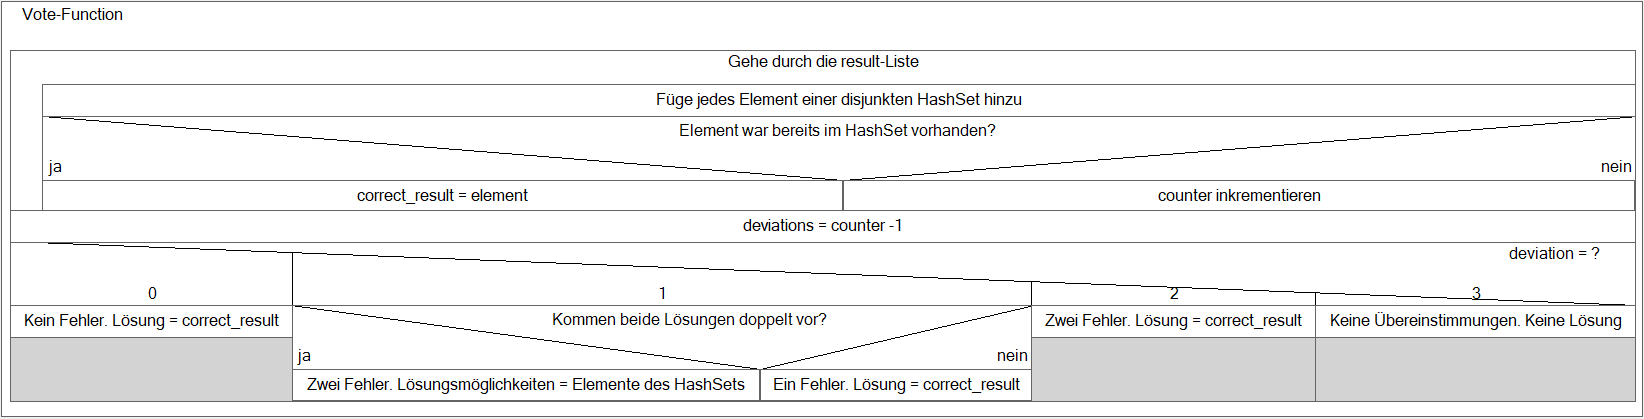
\includegraphics[width=1\linewidth]{images/vote_function_struktogramm.PNG}
    \caption{Struktogramm \textit{vote()}-Funktion}
    \label{fig:vote}
\end{figure}


 Im ersten Schritt wird in einer Schleife die Ergebnis Liste durchgegangen. Pro Durchgang wird das jeweilige Element einem disjunkten HashSet hinzugefügt und geprüft, ob dieses Element bereits im HashSet vorhanden ist. Falls ja, wird das Element in eine Ergebnisvariable (\textit{correct\textunderscore result}) überschrieben, anderenfalls wird ein Zähler inkrementiert. Durch den Zähler kann nun die Abweichung ermittelt werden, indem der Zähler dekrementiert wird (Zähler inkrementiert in der Schleife mindestens einmal). Über eine Switch-Anweisung wird nun diese Abweichung geprüft und dem Benutzer das Ergebnis mitgeteilt:
 
 \begin{itemize}
     \item Abweichung = 0: Alle Systeme übermitteln das gleiche Ergebnis. Kein Fehler aufgetreten. Als Lösung wird die Ergebnisvariable \textit{correct\textunderscore result} angezeigt.
     \item Abweichung = 1 (Spezialfall): Hier muss zunächst geprüft werden, ob die zwei verschiedenen Ergebnisse doppelt vorkommen.
     \begin{itemize}
         \item Falls ja: Keine eindeutige Lösung, da zwei verschiedenen Ergebnisse doppelt vorkommen. Als zwei Lösungsmöglichkeiten werden die Elemente des HashSets angezeigt.
         \item Falls nein: Drei Systeme übermitteln das gleiche Ergebnis. Ein Fehler ist aufgetreten. Als Lösung wird die Ergebnisvariable \textit{correct\textunderscore result} angezeigt.
     \end{itemize}
     \item Abweichung = 2: Zwei Systeme übermitteln das gleiche Ergebnis. Die anderen zwei Systeme unterscheiden sich im Ergebnis. Zwei Fehler aufgetreten. Als Lösung wird die Ergebnisvariable \textit{correct\textunderscore result} angezeigt.
     \item Abweichung = 3: Keine Übereinstimmung der Systeme. Mehrere Fehler aufgetreten.
\end{itemize}
	
Beim Spezialfall Abweichung = 1 muss geprüft werden, ob die verschiedenen Ergebnisse doppelt vorkommen. Diese Prüfung erfolgt in einer separaten Methode \textit{handle\textunderscore special\textunderscore case()}, welche ein Boolean zurückgibt. Diese Methode wurde in Unit-Tests getestet. Hierbei wurden die beiden Fälle „Ergebnisverhältnis 2:2“ und „Ergebnisverhältnis 1:3“ geprüft. Für die Tests wurde das JUnit Jupiter Modul verwendet.


\section{Implementierung der einzelnen Calculators}
Die Implementierung der Calculators ist in den folgenden Abschnitten beschrieben. Bei der Implementierung wurde darauf geachtet, dass nicht alle Calculators gleich implementiert sind, da dies dem Sinn der 2004-Architektur nicht entsprechen würde. Alle Calculators besitzen ihre eigenen Unit-Tests. 

\chapter{Calculator 1 (Bearbeiter: 8540946)}
\begin{lstlisting}[language=Java,basicstyle=\scriptsize, caption= Calculator 1]
public class Calculator1 implements ICalculator {
    private double _value1;
    private double _value2;
    private Operator _operator;

    public Calculator1(double value1, double value2, Operator Operator){
        this._value1 = value1;
        this._value2 = value2;
        this._operator = Operator;
    }

    @Override
    public double getResult() {
        double result = 0;
        switch (this._operator){
            case PLUS:
                result = add();
                break;
            case MINUS:
                result = subtract();
                break;
            case DIV:
                result = divide();
                break;
            case MULT:
                result = multiply();
                break;
        }
        return result;
    }

    private double add(){
        return this._value1 + this._value2;
    }

    private double subtract(){
        return this._value1 - this._value2;
    }

    private double divide(){
        return  this._value1 / this._value2;
    }

    private double multiply(){
        return this._value1 * this._value2;
    }
}
\end{lstlisting}
Die Klasse \textit{Calculator1} implementiert das Interface \textit{ICalculator} und besitzt drei Attribute vom Typ \textit{double}: \textit{\textunderscore value1}, \textit{\textunderscore value2} und \textit{\textunderscore operand}.\\
Dem Konstruktor der Klasse werden die Eingabeparameter value1, value2 und operand übergeben und dieser setzt die Klassenattribute gleich der Eingabeparameter.\\
Neben den drei Attributen besitzt die Klasse die vier private Methoden \textit{add()}, \textit{subtract()}, \textit{multiply()} und \textit{divide()}.
Diese sind Hilfsfunktionen, um aus den \textit{values} das Ergebnis zu berechnen.
Welche dieser Methoden aufgerufen wird, hängt von dem Operator ab.\\
Dieser wird geprüft, wenn der Nutzer die Methode \textit{getResult()} aufruft.
Die Methode \textit{getResult()} implementiert die entsprechende Methode des Interfaces.
Über die switch-Anweisung wird die zu dem jeweiligen Operator passende Methode zur Berechnung aufgerufen und am Ende wird das Resultat zurückgegeben.
Für die jeweilige Berechnung werden die vier Methoden \textit{add()}, \textit{subtract()}, \textit{multiply()} und \textit{divide()} aufgerufen, die auf die Klassenattribute zugreifen und entsprechend das Ergebnis berechnen und zurückgeben.\\
Das zurückgegebene Ergebnis wird in der lokalen Variable \textit{result} der Methode \textit{getResult()} gespeichert und die Methode gibt den Wert dieser Variable zurück.
\chapter{Calculator 2 (Bearbeiter: 6430174)}
\begin{lstlisting}[language=Java,basicstyle=\scriptsize, caption= Calculator 2]
public class Calculator2 implements ICalculator{

    private double result;

    public Calculator2 (double first_value, double sec_value, Operator Operator)
    {
        if (Operator == Operator.PLUS){
            result = first_value + sec_value;
        }
        else if (Operator == Operator.MINUS){
            result = first_value - sec_value;
        }
        else if (Operator == Operator.MULT){
            result = first_value * sec_value;
        }
        else if (Operator == Operator.DIV) {
            result = first_value / sec_value;
        }
    }

    public double getResult() {
        return result;
    }
}
\end{lstlisting}
Der \textit{Calculator2} implementiert das Interface \textit{ICalculator}. Die Klasse \textit{Calculator2} hat ein privates Attribut result vom Typ double. 
Der Konstruktor der Klasse übergibt die Eingabeparameter an das Calculator-Objekt. Die Eingabeparameter sind: Wert 1, Wert 2 und der Operator. Im Konstruktor wird direkt mittels der Eingabeparameter das Ergebnis berechnet. Dafür wird mit If-Abfragen der Operand ausgemacht und entsprechend das Ergebnis berechnet. Das Ergebnis wird dem Klassenattribut result zugewiesen.
Die Klasse verfügt außerdem über die öffentliche Methode \textit{getResult()}, die die gleichnamige Methode des Interfaces implementiert. Die Methode gibt den Wert des Attributs result zurück.

\chapter{Calculator 3 (Bearbeiter: 6274958)}

\begin{lstlisting}[language=Java,basicstyle=\scriptsize, caption= Calculator 3]
public class Calculator3 implements ICalculator{

    private double result;

    public Calculator3 (double value_one, double value_two, Operator Operator)
    {
        switch (Operator){
            case PLUS:
                result = value_one + value_two;
                break;
            case MINUS:
                result = value_one - value_two;
                break;
            case MULT:
                result = value_one * value_two;
                break;
            case DIV:
                result = value_one / value_two;
                break;
        }
    }

    public double getResult() {
        return result;
    }
}
\end{lstlisting}

Im Folgenden wird das System Nummer 3 der 2003-Architektur beschrieben. Hierfür wurde, wie auch bei den anderen Systemen, eine eigene Klasse erstellt, welche das Interface \textit{ICalculator} implementiert. Dem Konstruktor der Klasse werden zwei Werte und ein Operand übergeben. Die Methode basiert auf einer Switch-Anweisung, welche den Inhalt des übergebenen Operanden prüft. Hierbei können die vier Fälle der Operanden (\textit{PLUS, MINUS, MULT, DIV}) in der Anweisung eintreten. Durch die Auswahl wird entschieden, welche Berechnungsvorschrift für die Verrechnung der zwei übergebenen Werte verwendet werden soll.  Das Ergebnis der Berechnung wird in eine private Ergebnisvariable geschrieben. Mittels der Methode \textit{getResult()}, welche den Inhalt der Ergebnisvariable zurückgibt, kann außerhalb der Klasse auf der Ergebnis zugegriffen werden. 


Um die ganze Methode und dessen Berechnungsvorschriften zu testen, wurden Unit-Tests geschrieben. Zu jeder Berechnungsvorschrift wurden jeweils zwei Tests geschrieben. Hier wurde besonders geschaut, dass Spezialfälle, wie zum Beispiel Dezimalzahlen (Kommazahlen) oder negative Zahlen, in den Tests abgedeckt werden. Für die Tests wurde das JUnit Jupiter Modul verwendet.


\chapter{Calculator 4 (Bearbeiter: 5060216)}

Diese Klasse wurde nach der testgetriebenen Methode entwickelt. Um bei den Unit Tests ausschließlich einzelne Methoden zu testen, wurde jede einzelne Funktionalität in einer eigenen Methode ausgelagert. Insgesamt gibt es eine Methoden für jede Rechenoperation, die alle das gleiche Interface besitzen – keine Übergabeparameter, keine Rückgabeparameter. Des Weiteren wurde die ICalculator \textit{getResult} Methode implementiert, welche das berechnete Ergebnis zurückgibt.

Da alle Methoden die erste und zweite Zahl zur Berechnung benötigen, werden die Zahlen nach Aufruf des Konstruktors zunächst in private static Variablen gespeichert. Aus Gründen der Performance, wird nicht jede Methode mit der ersten und zweiten Zahl aufgerufen. Die Variablen sind static, da diese nur einmal bei Konstruktoraufruf bzw. nach der Berechnung gesetzt werden. Da die Klasse jedoch nicht static ist, hat dies nur bedingt eine Relevanz, bietet allerdings mehr Spielräume für spätere Refactoring-Maßnahmen.
In einem \textit{switch-case} wird der dem Konstruktor übergebene Enum-Operand ausgewertet und die zugehörige Rechenoperation-Methode aufgerufen. Jede Rechenoperation-Methode speichert das berechnete Ergebnis in eine Variable, welche durch die getResult Methode zurückgegeben wird.

Die Divisionsmethode besitzt zusätzlich zu der Rechenoperation noch ein Abfangen des „Zero Divsion Errors“, um zu verhindern, dass das Programm bei einer ungültigen Rechenoperation crasht. In diesem Fall wird der Nutzer über die ungültige Rechenoperation informiert und das Ergebnis gleich Null gesetzt.

Die Test Klasse wurde mit dem jUnit Modul entwickelt. Da in der Klasse mit doubles gearbeitet wird treten Rundungsfehler aufgrund der Tatsache, dass mit floating point numbers gerechnet wird, auf. Dadurch können manche Tests scheitern obwohl die Methoden das eigentliche richtige Ergebnis berechnet haben. Um diese Problemstellung zu lösen, wird der \textit{assertEqual}-Befehl verwendet um ein delta festzulegen, welches toleriert wird. Liegt das Ergebnis der Methode innerhalb dieses Toleranzbandes des Exaktwertes, gilt die Berechnung als korrekt.

Jede Operation wurde mit double Zahlen getestet und es wurde versucht möglichst viele Fälle zu testen. Jede Methode besitzt mindestens 4 Testfälle, die aus der folgenden Tabelle 1 zu entnehmen sind.

\begin{table}[H]
\centering
\begin{tabular}{c c c}
	Testfall & VZ 1. Nummer & VZ 2. Nummer\\
	\hline
	1 & + & +\\
	2 & + & -\\
	3 & - & +\\
	4 & - & -\\
	%\bottomrule 
\end{tabular}
\caption{Testfälle}
\end{table}

Des Weiteren wurde bei der Divisionsmethode getestet, ob das Abfangen des Sonderfalls (\textit{second\textunderscore num=0}) korrekt funktioniert. Alle Tests laufen erfolgreich durch und beweisen die korrekte Implementierung.

\chapter{Anhang}
\begin{figure}[H]
\centering
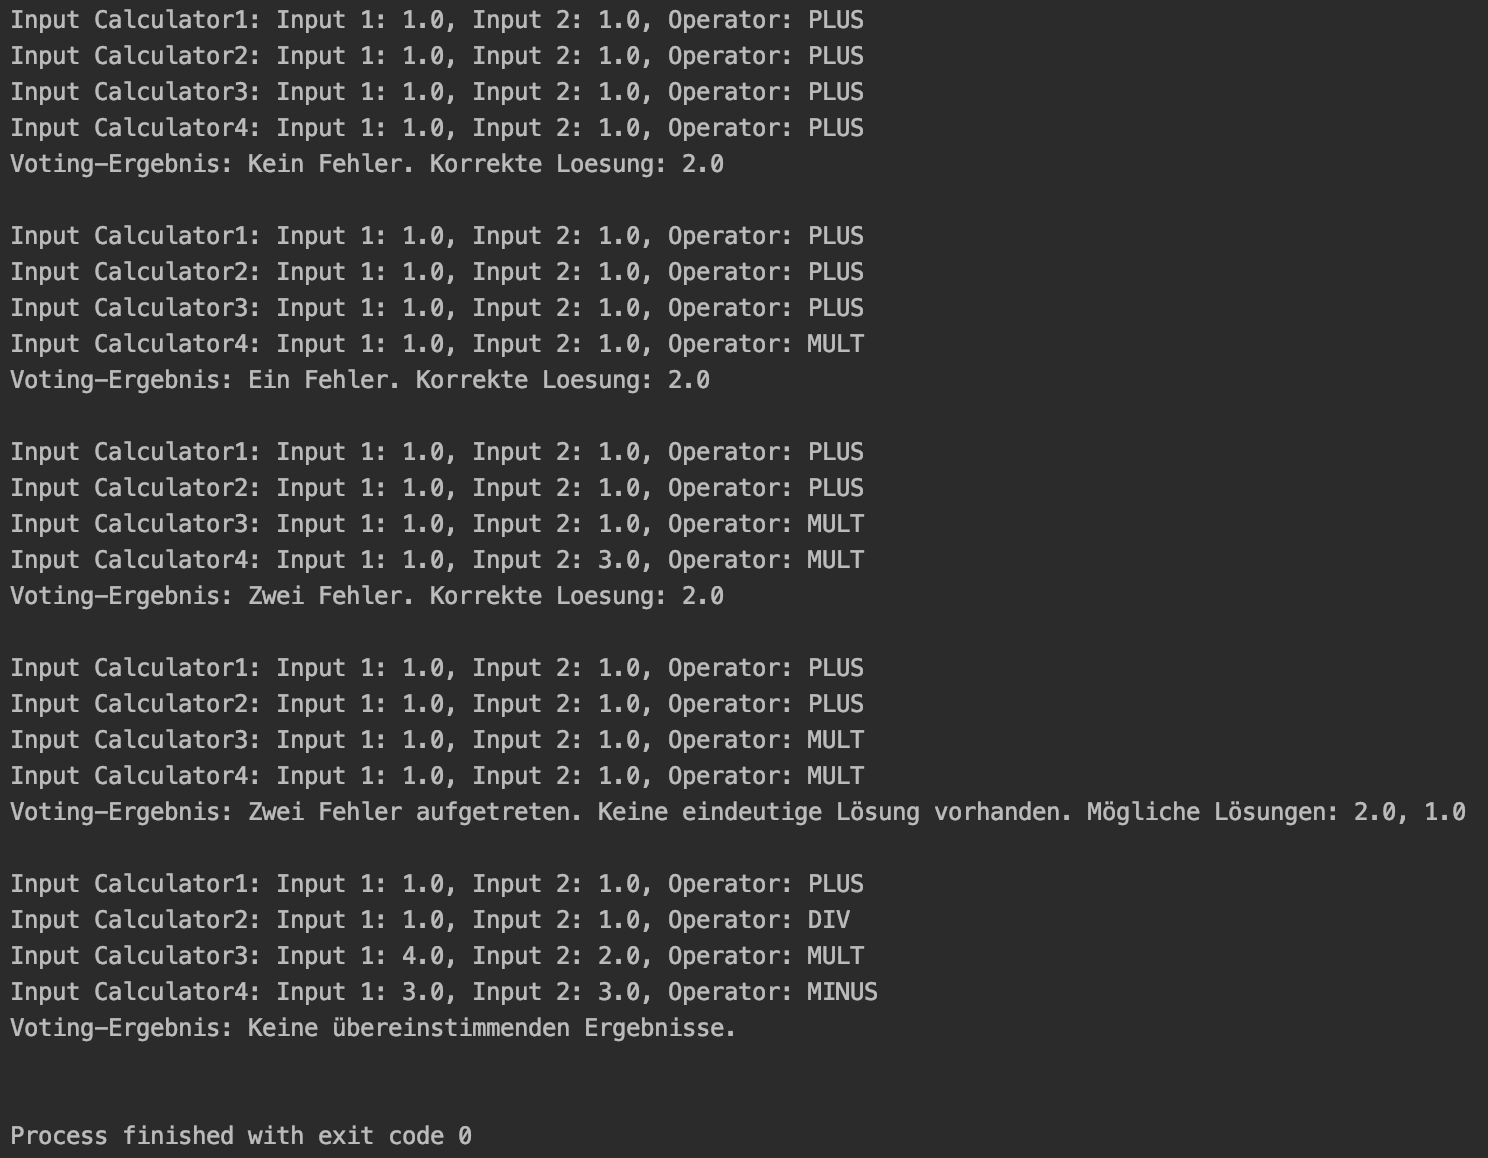
\includegraphics[width=1\textwidth]{images/tool_output.png}
\caption{Ausgabe des Tools}
\end{figure}
